\section{SAT}

	\begin{frame}[plain]
		\vfill
		\centering
		\begin{beamercolorbox}[sep=8pt,center,shadow=true,rounded=true]{title}
			\textbf{\usebeamerfont{title}\insertsectionhead}\par%
			\color{polimiblue}\noindent\rule{10cm}{1pt} \\
			\textbf{The SATisfiability problem}
		\end{beamercolorbox}
		\vfill
	\end{frame}

	\subsection{Problem Definition}
		\begin{frame}{Problem Definition}
			\small
			 Let $X\equiv\{x_1, x_2, ..., x_n\}$ be a set\\
			 \vspace{0.1cm}
			 Then $x_k$ and its negations $\overline{x}_k$ are called literals and the set of all literals is denoted by $X^{'}=\{x_1, \overline{x}_1, ..., x_n, \overline{x}_n\}$\\
			 \vspace{0.1cm}
			 The set of all subsets of $X^{'}$ is denoted by $\mathcal{F}(X^{'})$ and an element $C\in\mathcal{F}(X^{'})$ is called a clause\\
			 
			 \vspace{0.3cm}
			 
			 \textbf{SAT problem:} \emph{Given a set $X=\{x_1, x_2, ..., x_n\}$ and a set of clauses $\mathcal{C}=\{C_1, C_2, ..., C_m\}$ of clauses, determine whether $\mathcal{C}$ is satisfiable or not.\\}
			 
			 \vspace{0.3cm}
			 
			 In the literature we find the problem typically identified as k-SAT where we need to consider:
			 \begin{itemize}
			 	\item[1.] The number of variables on which the problem is defined: \textbf{n}
			 	
			 	\item[2.] The number of clauses on which the problem is defined: \textbf{m}
			 	
			 	\item[3.] The maximal length of the clauses in the problem: \textbf{k}
			 \end{itemize}
		\end{frame}
	
		\begin{frame}{SAT example}
			\small
			Consider the following two clauses defining a 3-SAT problem over the variables $x_1, x_2, x_3$:
			\begin{center}
				$C_1=\{\overline{x}_1, x_2, x_3\}$
				\hspace{0.5cm}
				$C_2=\{x_1, \overline{x}_2, x_3\}$
			\end{center} 
			Corresponding to the \emph{Conjunctive Normal Form}:
			\begin{equation*}
				\centering
				CNF=(\overline{x}_1\lor x_2\lor x_3)\land(x_1\lor\overline{x}_2\lor x_3)
			\end{equation*}
			\vspace{1cm}
			\begin{minipage}{0.38\textwidth}
				That we represented in a quantum circuit, by exploiting the relations between the quantum and classical operations, as represented in the picture on the right
				\vspace{1.2cm}
			\end{minipage}
			\hfill
			\begin{minipage}{0.6\textwidth}
				\centering
				\begin{figure}[h]
					\centering
					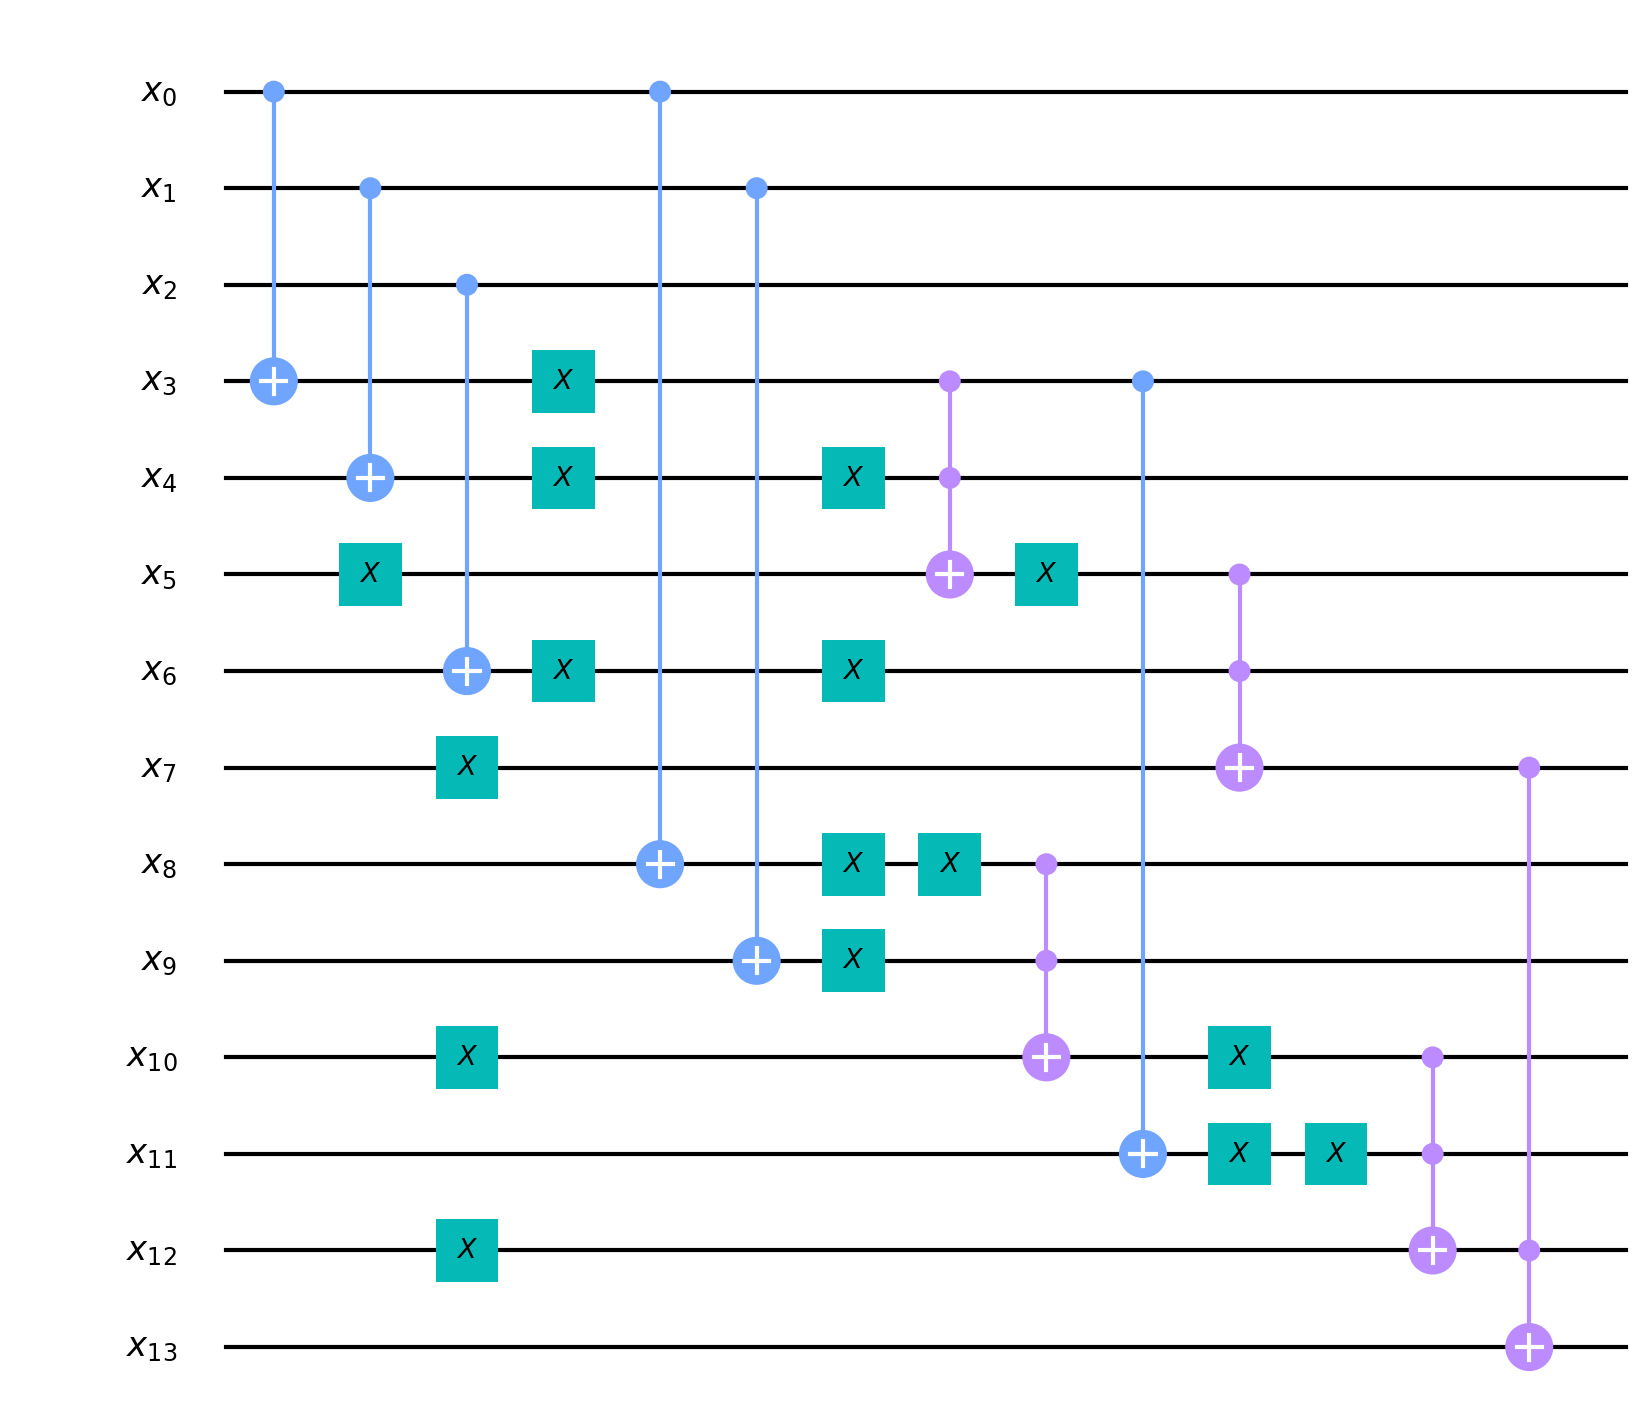
\includegraphics[scale=0.19]{exampleSAT.png}
				\end{figure}
			\end{minipage}
		\end{frame}
	
	
	\subsection{Classical Solver}
		%\begin{frame}{Classical Solver}
		
		%\end{frame}
	
	\subsection{Quantum Solver}
		%\begin{frame}{Quantum Solver}
			
		%\end{frame}
	
	\subsection{Classic vs. Quantum}
		%\begin{frame}{Classic vs. Quantum}
		
		%\end{frame}
		
	\subsection{Conclusions}
		%\begin{frame}{Conclusions}
		
		%\end{frame}
		
	